\documentclass[12pt]{article}

\usepackage[T1]{fontenc}
\usepackage[utf8]{inputenc} % L'encodage du document
\usepackage[french]{babel} % Des options supplémentaires pour que le document soit en français (noms de sections, etc.)
\usepackage{geometry}
\geometry{hscale=0.80,vscale=0.80,centering} % Permet de définir les marges (ici 10% de chaque côté)
\usepackage{amsmath}
\usepackage{amssymb}
\usepackage{amsthm} % For theorem-like environments
\usepackage{graphicx} % Ajout du package graphicx
\usepackage{minted}
\usepackage{fixltx2e}
\usepackage{array}
\usepackage{lettrine}
\usepackage{tikz}
\usepackage[ruled,linesnumbered,french,onelanguage]{algorithm2e}
\usepackage{algpseudocode}
\usetikzlibrary{angles,quotes}

\newcolumntype{C}[1]{>{\centering\arraybackslash}m{#1}}
\newcolumntype{L}[1]{>{\raggedright\arraybackslash}m{#1}}
\newcolumntype{N}{@{}m{0pt}@{}}

\newcounter{definitioncounter}
\renewcommand{\thedefinitioncounter}{\arabic{definitioncounter}}

\newcommand{\definition}[1]{%
    \par\noindent\textbf{Définition \refstepcounter{definitioncounter}\thedefinitioncounter.} #1 \vspace{0.5\baselineskip}
}

\newcommand{\fig}[1]{
    F\resizebox{!}{1.3ex}{IGURE} #1
}

\newcounter{propositioncounter}
\renewcommand{\thepropositioncounter}{\arabic{propositioncounter}}

\newcommand{\proposition}[1]{%
    \par\noindent\textbf{Proposition \refstepcounter{propositioncounter}\thepropositioncounter.} #1 \vspace{0.5\baselineskip}
}

\setlength{\parindent}{15pt} % Fixe l'indentation en début de paragraphe
\setlength{\parskip}{10pt} % Fixe l'espacement entre paragraphes

\begin{document}
\title{Simuler les feux de forêt}
\date{\today}
\author{Victor Sarrazin}

\maketitle

\section*{Introduction}

Avec le changement climatique, les feux de forêt sont de plus en plus fréquents et dévastateurs, à l'image de ceux en Californie en janvier 2025.

Dans ce cadre, les modélisations informatiques des feux de forêt permettent de simuler leur évolution et ainsi de prévoir les zones à risque. Elles offrent également la possibilité de tester l'impact de certaines transformations sur ces incendies, afin d'identifier des moyens de réduire les conséquences des catastrophes sans dénaturer les forêts.

\section{Automates cellulaires}

Pour réaliser nos modélisations, nous allons utiliser des automates cellulaires. Ces outils permettent de représenter des systèmes avec des interactions locales entre les éléments qui les constituent. Les automates cellulaires ont notamment été popularisés avec \textit{Le~Jeu~de~la~Vie} de \textit{Conway}.

\definition{Un automate cellulaire est la donnée d'un triplet $(Q, M, f)$ avec :\begin{itemize}
    \item $Q$ un ensemble d'états
    \item $M$ une matrice de taille $n \times m$, où chaque $m_{i,j}$ représente une cellule de la grille
    \item $f : \mathcal{M}_{n,m}(Q) \longrightarrow \mathcal{M}_{n,m}(Q)$ une \textit{fonction de transition} qui à une grille renvoie la grille suivante
\end{itemize}}

La définition de la fonction de transition dépend donc du type de voisinage considéré. Il existe deux principaux types de voisinages : celui de \textit{von Neumann} et celui de \textit{Moore}. Nous avons choisi d'utiliser le voisinage de \textit{Moore} pour nos modélisations pour prendre en compte le plus d'intéractions possibles, celui de \textit{von Neumann} étant plus limitatif, notamment en ce qui concerne les interactions diagonales.

\definition{Le voisinage de \textit{Moore} est composé de la cellule centrale et de ses 8 voisins adjacents (horizontalement, verticalement et diagonalement).}

\begin{figure}[!ht]
    \centering
    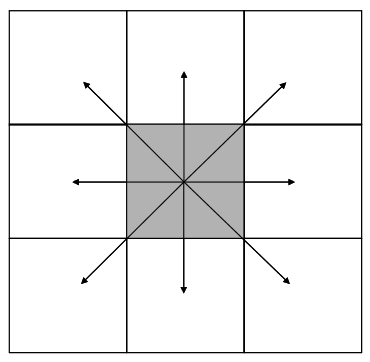
\includegraphics[width=0.20\linewidth]{pictures/moore.png}
    \caption{Voisinage de Moore}
    \label{fig:enter-label}
\end{figure}

Il serait possible dans une optique d'avoir des modèles encore plus précis d'utiliser des voisinages de \textit{Moore} étendus, avec plusieurs rayons de voisins. Cependant par souci de simplicité nous nous sommes restreints à un rayon.

% \subsection{Représentation d'un forêt}

% Afin de représenter une forêt avec un automate cellulaire, nous avons défini une liste d'états que les cellules pouvaient prendre.

% \definition{Les états possibles sont :
% \begin{itemize}
%     \item Arbres
%     \item Arbres denses
%     \item Champs
%     \item Feu
%     \item Case brûlée\textsuperscript{*}
%     \item Eau\textsuperscript{*}
% \end{itemize}
% A noter que les cases $(*)$ ne peuvent brûler.}

% Nous avons choisi de travailler avec une matrice de taille $256 \times 256$ pour des raisons techniques : au-delà le temps de calcul devenait trop long, et l'ajout de lignes/colonnes ne représentait pas un intérêt suffisant au regard du temps de calcul que cela impliquait.

\section{Modèle d'Alexandridis}

Dans un premier temps, il est possible de réaliser une modélisation simple des feux de forêt en associant à chaque cellule une probabilité fixe de s'enflammer si l'un de ses voisins est en feu. Une telle tentative a donné des résultats mitigés. C'est pourquoi l'objectif de cette deuxième partie est de présenter un modèle plus avancé de modélisation des feux de forêts, appelé modèle d'\textit{Alexandridis}.

\subsection{Présentation du modèle}

Le modèle d'\textit{Alexandridis} prend en compte divers phénomènes pour simuler la propagation des incendies. Par la suite, nous avons choisi de nous concentrer sur la densité de végétation, le type de végétation ainsi que le vent dans la zone. Le modèle original prend également en considération l'élévation du terrain.

\proposition{On utilise les règles de transition suivantes, pour $(i,j) \in \mathbb{N}^2$, $t \in \mathbb{N}$ :
\begin{itemize}
    \item Si $m_{i,j} (t) = $ \mintinline{latex}{feu} alors $m_{i,j} (t+1) = $ \mintinline{latex}{brulé}
    \item Si $m_{i,j} (t) = $ \mintinline{latex}{feu} alors $m_{i \pm 1,j \pm 1} (t+1) = $ \mintinline{latex}{feu} avec une probabilité $p_b$
    \item Si $m_{i,j} (t) = $ \mintinline{latex}{brulé} alors $m_{i,j} (t+1) = $ \mintinline{latex}{brulé}
\end{itemize}}

\proposition{La probabilité $p_b$ qu'une cellule brûle est définie par
$p_b = p_h (1 + p_{veg}) (1 + p_{den}) p_{vent}$ avec $p_h = 0.27$ une constante, et $p_{veg}$ et $p_{den}$ des coefficients relatifs au type de cellule.
}

\begin{figure}[!ht]
    \centering
    \renewcommand{\arraystretch}{2}
    \setlength{\extrarowheight}{-3pt}
    \begin{tabular}{ |>{\centering\arraybackslash}p{4cm}|>{\centering\arraybackslash}p{2cm}|>{\centering\arraybackslash}p{2cm}| }
        \cline{2-3}
        \multicolumn{1}{c|}{} & $p_{veg}$ & $p_{den}$ \\
        \hline 
        Arbres & $0.3$ & $0.3$ \\ 
        \hline
        Arbres denses & $0.3$ & $0$ \\ 
        \hline
        Champs & $-0.1$ & $0$ \\
        \hline 
    \end{tabular}
    \caption{Probabilités $p_{veg}$ et $p_{den}$ selon le type de végétation}
\end{figure}

\proposition{La probabilité $p_{vent}$ liée au vent est définie par
\\ $p_{vent} = \exp (0.045 v) \times \exp (0.131 v \times (\cos (\theta) - 1))$ avec $\theta$ l'angle entre la propagation du feu et la direction du vent, et $v$ la vitesse du vent (en $m/s$)
}

\begin{figure}[!ht]
    \centering
    \begin{tikzpicture}[> = stealth]
        \coordinate (a) at (1,4);
        \coordinate (b) at (2,5);
        \coordinate (c) at (5,4);
        \coordinate (d) at (6,4);
        \coordinate (e) at (9,5);
        \coordinate (f) at (10,4);
        
        \draw pic[draw,fill=green!30,angle radius=1cm,"$\theta_1$" shift={(6mm,1mm)}] {angle=c--a--b};
        \draw pic[draw,fill=green!30,angle radius=2cm,"$\theta_2$" shift={(6mm,1mm)}] {angle=f--d--e};
        
        \draw[ultra thick,red, ->]  (a) -- node[above left] {\normalsize Vent} (b);
        \draw[ultra thick,blue,->]  (a) -- node[below] {\normalsize Propagation du feu} (c);

        \draw[ultra thick,red, ->]  (d) -- node[above left] {\normalsize Vent} (e);
        \draw[ultra thick,blue,->]  (d) -- node[below] {\normalsize Propagation du feu} (f);
    \end{tikzpicture}
    \caption{Configurations de vent}
\end{figure}

On a $\theta_1 > \theta_2$ et une vitesse plus élevée dans la seconde situation, ainsi la probabilité $p_{vent}$ sera plus élevée dans la seconde situation.

\subsection{Résultats}

Voici un résultat de modélisation de feu, avec un vent de $15 m/s$ orienté vers l'est :

\begin{figure}[!ht]
    \centering
    \begin{minipage}{0.50\textwidth}
      \centering
      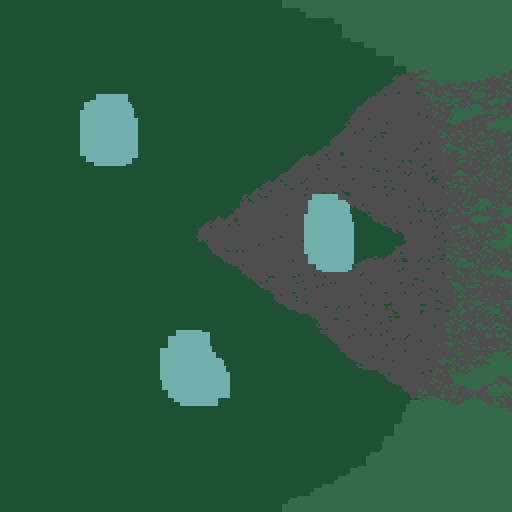
\includegraphics[width=.6\linewidth]{pictures/model2/land_200_wind_notdense.png}
      \caption{Simulation Alexandridis}\label{Fig:Data3}
    \end{minipage}\hfil
 \end{figure}

\section{Hashlife}

Afin de réaliser des modélisations plus conséquentes (notamment en augmentant la taille de la grille), il faut trouver une manière de réduire le nombre de calculs. C'est l'objectif de l'algorithme de mémoïsation \mintinline{latex}|Hashlife|, notamment utilisé dans le logiciel \mintinline{latex}|Golly|\footnote{https://golly.sourceforge.io/} pour les simulations du \textit{Jeu de la Vie} de \textit{Conway}.

Au lieu de calculer chaque cellule indépendamment, l'algorithme considère des groupements de cellules, dits \textit{macro-cellules}, de taille $2^n \times 2^n$, que l'on peut redécouper en 4 quadrants de taille $2^{n-1} \times 2^{n-1}$ (partie en bleu sur la figure).

On appelle \textit{résultat} la macro-cellule centrale de taille $2^{n-1} \times 2^{n-1}$ (partie en rouge sur la figure).

\begin{figure}[!ht]
    \centering
        \begin{tikzpicture}[> = stealth]
            \draw[step=0.25cm,color=gray] (-1,-1) grid (1,1);
            \draw[fill=blue,fill opacity=0.6,draw=black] (-0.75,-0.75) rectangle ++(1.5,1.5);
            \draw[step=1cm,color=black] (-1,-1) grid (1,1);
            \draw[step=0.25cm,color=gray] (2,-1) grid (4,1);
            \draw[step=1cm,color=black] (2,-1) grid (4,1);
            \draw[fill=red,fill opacity=0.6,draw=black] (2.5,-0.5) rectangle ++(1,1);
        \end{tikzpicture}
    \caption{Une macro-cellule de taille $2^{3} \times 2^{3}$}
\end{figure}

Ce découpage en macro-cellule permet de calculer le résultat sans considérer aucune information extérieure à la macro-cellule pendant $2^{n-2}$ unités de temps. Ce calcul est fait récursivement selon deux cas :

Soit $n = 2$, le résultat est composé d'uniquement $4$ cellules, dans ce cas on le calcule directement en appliquant les règles de notre automate cellulaire.

Sinon $n > 2$, on a donc $4$ quadrants de taille $2^{n-1} \times 2^{n-1}$ pour lesquels on calcule récursivement leur résultat (ici en bleu). Ensuite il faut calculer les $5$ macro-cellules de taille $2^{n-2} \times 2^{n-2}$ (en rouge) en considérant les macro-cellules de taille $2^{n-1} \times 2^{n-1}$ associées (exemple en vert).

Enfin après ces précalculs effectués, on peut calculer les quatre macro-cellules de taille $2^{n-2}$ (en jaune) afin d'obtenir le résultat que l'on recherche.

\begin{figure}[!ht]
    \centering
        \begin{tikzpicture}[> = stealth]
            \draw[fill=none,draw=black] (-1,-1) rectangle ++(2,2);
            \draw[step=1cm,color=black] (-1,-1) grid (1,1);
            \draw[fill=blue,fill opacity=0.6,draw=black] (-0.75,-0.75) rectangle ++(0.5,0.5);
            \draw[fill=blue,fill opacity=0.6,draw=black] (0.25,-0.75) rectangle ++(0.5,0.5);
            \draw[fill=blue,fill opacity=0.6,draw=black] (-0.75,0.25) rectangle ++(0.5,0.5);
            \draw[fill=blue,fill opacity=0.6,draw=black] (0.25,0.25) rectangle ++(0.5,0.5);
            \draw[step=1cm,color=black] (2,-1) grid (4,1);
            \draw[fill=gray,fill opacity=0.6,draw=black] (2.25,-0.75) rectangle ++(0.5,0.5);
            \draw[fill=gray,fill opacity=0.6,draw=black] (3.25,-0.75) rectangle ++(0.5,0.5);
            \draw[fill=gray,fill opacity=0.6,draw=black] (2.25,0.25) rectangle ++(0.5,0.5);
            \draw[fill=gray,fill opacity=0.6,draw=black] (3.25,0.25) rectangle ++(0.5,0.5);
            \draw[fill=red,fill opacity=0.6,draw=black] (2.25,-0.25) rectangle ++(0.5,0.5);
            \draw[fill=red,fill opacity=0.6,draw=black] (2.75,-0.75) rectangle ++(0.5,0.5);
            \draw[fill=red,fill opacity=0.6,draw=black] (2.75,0.25) rectangle ++(0.5,0.5);
            \draw[fill=red,fill opacity=0.6,draw=black] (3.25,-0.25) rectangle ++(0.5,0.5);
            \draw[fill=red,fill opacity=0.6,draw=black] (2.75,-0.25) rectangle ++(0.5,0.5);
            \draw[step=1cm,color=black] (5,-1) grid (7,1);
            \draw[fill=green,fill opacity=0.6,draw=black] (5,-0.5) rectangle ++(1,1);
            \draw[fill=red,fill opacity=0.6,draw=black] (5.25,-0.25) rectangle ++(0.5,0.5);
            \draw[step=1cm,color=black] (8,-1) grid (10,1);
            \draw[fill=yellow,fill opacity=0.6,draw=black] (8.5,-0.5) rectangle ++(0.5,0.5);
            \draw[fill=yellow,fill opacity=0.6,draw=black] (9,-0.5) rectangle ++(0.5,0.5);
            \draw[fill=yellow,fill opacity=0.6,draw=black] (8.5,0.0) rectangle ++(0.5,0.5);
            \draw[fill=yellow,fill opacity=0.6,draw=black] (9,0.0) rectangle ++(0.5,0.5);
        \end{tikzpicture}
    \caption{Calcul dans le cas $n > 2$}
\end{figure}

Si dans le cas $n=2$ on fait le même nombre d'opérations que dans la simulation naïve, le cas $n>2$ réalise une réelle économie de calcul.

Mais \mintinline{latex}|Hashlife| n'est pas uniquement une réduction du nombre de calculs dans les itérations. En effet l'algorithme exploite le fait que les automates cellulaires présentent des répétitions de motifs durant l'exécution, notamment avec les \textit{gliders} dans \textit{Le~Jeu~de~la~Vie} volant jusqu'aux bordures (infinies) de la grille :

\begin{figure}[!ht]
    \centering
        \begin{tikzpicture}[> = stealth]
            \draw[step=0.4cm,color=gray] (0,0) grid (2,2);
            \draw[fill=black,draw=black] (0.4,0.8) rectangle ++(0.4,0.4);
            \draw[fill=black,draw=black] (0.8,0.4) rectangle ++(0.4,0.4);
            \draw[fill=black,draw=black] (1.2,0.4) rectangle ++(0.4,1.2);
            \draw[step=2cm,color=black] (0,0) grid (2,2);
        \end{tikzpicture}
    \caption{Un \textit{glider}}
\end{figure}

C'est pourquoi \mintinline{latex}|Hashlife| réalise aussi une mémoïsation des résultats de chaque quadrant à l'aide d'une table de hashage, d'où le nom de l'algorithme. Celà permet de réutiliser au maximum les calculs et d'éviter de recalculer les situations récurrentes.

Si \mintinline{latex}|Hashlife| permet de réduire drastiquement le temps de calcul pour des grandes grilles et de s'affranchir de bornes de ces dernières en exploitant les motifs qui se répètent, il existe toujours des cas dégénérés où l'algorithme a une complexité similaire à celui naïf si les motifs ne se répètent jamais\footnote{L'algorithme \mintinline{latex}|Quicklife| permet de résoudre ce problème}.

\section{Conclusion}

Les automates cellulaires permettent de simuler de nombreux systèmes avec des interactions tels que les feux de forêt. Cependant pour réussir à avoir des simulations d'une taille convaincante (et dans un temps raisonnable) il faut implémenter des algorithmes plus poussés tels que \mintinline{latex}|Hashlife|.

% \subsection{Pseudo code}

% Une implémentation en pseudo-code de \mintinline{latex}|Hashlife| est la suivante :

% \begin{figure}[!ht]
%     \begin{minipage}{0.90\textwidth}
%       \centering
% \begin{algorithm}[H]
% \SetKwFunction{Hashlife}{Hashlife}
% \SetKwData{hashtable}{hashtable}
% \SetKwData{cellule}{cellule}
% \SetKwData{n}{n}
% \SetKwData{nouvellecellule}{nouvelle\_cellule}
% \SetKwData{enfantun}{enfant1}
% \SetKwData{enfantdeux}{enfant2}
% \SetKwData{enfanttrois}{enfant3}
% \SetKwData{enfantquatre}{enfant4}
% \SetKwProg{Fn}{Fonction}{:}{}

% \DontPrintSemicolon % Suppress semicolons at the end of lines

% \caption{Hashlife}\label{alg:cap}
% \SetAlgoLined
% \Fn{\Hashlife{\cellule}}{
%     \If{\KwSty{hash}(\cellule) \KwSty{dans} \hashtable}{
%         \Return \hashtable[\KwSty{hash}(\cellule)]\;
%     }
%     \BlankLine
%     \nouvellecellule $\gets$ Cellule vide\;
%     \If{\cellule.\n = 2}{
%         \nouvellecellule $\gets$ Calcul du résultat $2 \times 2$\;
%     }
%     \Else{
%         \nouvellecellule.\enfantun $\gets$ \Hashlife{\cellule.\enfantun}\;
%         \nouvellecellule.\enfantdeux $\gets$ \Hashlife{\cellule.\enfantdeux}\;
%         \nouvellecellule.\enfanttrois $\gets$ \Hashlife{\cellule.\enfanttrois}\;
%         \nouvellecellule.\enfantquatre $\gets$ \Hashlife{\cellule.\enfantquatre}\;
%     }
%     \BlankLine
%     \hashtable[\KwSty{hash}(\cellule)] $\gets$ \nouvellecellule\;
%     \Return \nouvellecellule\;
% }
% \end{algorithm}
%     \end{minipage}
% \end{figure}

% \section{Bibliographie}

\end{document}